\scalebox{1.25}{
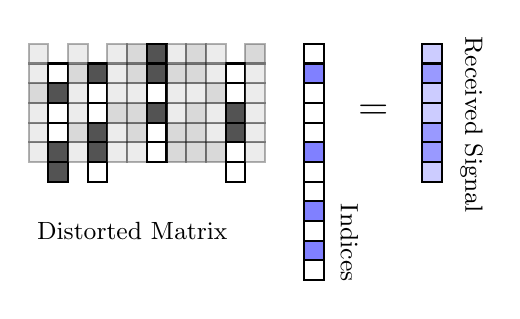
\begin{tikzpicture}
[font=\small, draw=black, line width=0.75pt,
entry0/.style={rectangle, draw, opacity=0.3, fill=lightgray, inner sep=0pt, minimum size=2.5mm},
entry1/.style={rectangle, draw, opacity=0.3, fill=gray, inner sep=0pt, minimum size=2.5mm},
entry00/.style={rectangle, draw, fill=white, inner sep=0pt, minimum size=2.5mm},
entry11/.style={rectangle, draw, fill=darkgray!90, inner sep=0pt, minimum size=2.5mm},
entry2/.style={rectangle, draw, fill=blue, inner sep=0pt, minimum size=2.5mm},
noentry/.style={rectangle, inner sep=0pt, minimum size=2.5mm},
symbol0/.style={rectangle, draw, fill=white, inner sep=0pt, minimum size=2.5mm},
symbol1/.style={rectangle, draw, fill=blue!50, inner sep=0pt, minimum size=2.5mm}]

\node[noentry] (m0000) at (0.00,0) {};
\node[entry11] (m0100) at (0.25,0) {};
\node[noentry] (m0200) at (0.50,0) {};
\node[entry00] (m0300) at (0.75,0) {};
\node[noentry] (m0400) at (1.00,0) {};
\node[noentry] (m0500) at (1.25,0) {};
\node[noentry] (m0600) at (1.50,0) {};
\node[noentry] (m0700) at (1.75,0) {};
\node[noentry] (m0800) at (2.00,0) {};
\node[noentry] (m0900) at (2.25,0) {};
\node[entry00] (m1000) at (2.50,0) {};
\node[noentry] (m1100) at (2.75,0) {};

\node[entry0] (m0001) at (0.00,0.25) {};
\node[entry11] (m0101) at (0.25,0.25) {};
\node[entry0] (m0201) at (0.50,0.25) {};
\node[entry11] (m0301) at (0.75,0.25) {};
\node[entry0] (m0401) at (1.00,0.25) {};
\node[entry0] (m0501) at (1.25,0.25) {};
\node[entry00] (m0601) at (1.50,0.25) {};
\node[entry1] (m0701) at (1.75,0.25) {};
\node[entry1] (m0801) at (2.00,0.25) {};
\node[entry1] (m0901) at (2.25,0.25) {};
\node[entry00] (m1001) at (2.50,0.25) {};
\node[entry0] (m1101) at (2.75,0.25) {};

\node[entry0] (m0002) at (0.00,0.50) {};
\node[entry00] (m0102) at (0.25,0.50) {};
\node[entry1] (m0202) at (0.50,0.50) {};
\node[entry11] (m0302) at (0.75,0.50) {};
\node[entry0] (m0402) at (1.00,0.50) {};
\node[entry1] (m0502) at (1.25,0.50) {};
\node[entry00] (m0602) at (1.50,0.50) {};
\node[entry1] (m0702) at (1.75,0.50) {};
\node[entry1] (m0802) at (2.00,0.50) {};
\node[entry0] (m0902) at (2.25,0.50) {};
\node[entry11] (m1002) at (2.50,0.50) {};
\node[entry0] (m1102) at (2.75,0.50) {};

\node[entry0] (m0003) at (0.00,0.75) {};
\node[entry00] (m0103) at (0.25,0.75) {};
\node[entry0] (m0203) at (0.50,0.75) {};
\node[entry00] (m0303) at (0.75,0.75) {};
\node[entry1] (m0403) at (1.00,0.75) {};
\node[entry1] (m0503) at (1.25,0.75) {};
\node[entry11] (m0603) at (1.50,0.75) {};
\node[entry0] (m0703) at (1.75,0.75) {};
\node[entry1] (m0803) at (2.00,0.75) {};
\node[entry0] (m0903) at (2.25,0.75) {};
\node[entry11] (m1003) at (2.50,0.75) {};
\node[entry0] (m1103) at (2.75,0.75) {};

\node[entry1] (m0004) at (0.00,1.00) {};
\node[entry11] (m0104) at (0.25,1.00) {};
\node[entry0] (m0204) at (0.50,1.00) {};
\node[entry00] (m0304) at (0.75,1.00) {};
\node[entry0] (m0404) at (1.00,1.00) {};
\node[entry0] (m0504) at (1.25,1.00) {};
\node[entry00] (m0604) at (1.50,1.00) {};
\node[entry0] (m0704) at (1.75,1.00) {};
\node[entry0] (m0804) at (2.00,1.00) {};
\node[entry1] (m0904) at (2.25,1.00) {};
\node[entry00] (m1004) at (2.50,1.00) {};
\node[entry0] (m1104) at (2.75,1.00) {};

\node[entry0] (m0005) at (0.00,1.25) {};
\node[entry00] (m0105) at (0.25,1.25) {};
\node[entry1] (m0205) at (0.50,1.25) {};
\node[entry11] (m0305) at (0.75,1.25) {};
\node[entry0] (m0405) at (1.00,1.25) {};
\node[entry1] (m0505) at (1.25,1.25) {};
\node[entry11] (m0605) at (1.50,1.25) {};
\node[entry1] (m0705) at (1.75,1.25) {};
\node[entry1] (m0805) at (2.00,1.25) {};
\node[entry0] (m0905) at (2.25,1.25) {};
\node[entry00] (m1005) at (2.50,1.25) {};
\node[entry0] (m1105) at (2.75,1.25) {};

\node[entry0] (m0006) at (0.00,1.5) {};
\node[noentry] (m0106) at (0.25,1.5) {};
\node[entry0] (m0206) at (0.50,1.5) {};
\node[noentry] (m0306) at (0.75,1.5) {};
\node[entry0] (m0406) at (1.00,1.5) {};
\node[entry1] (m0506) at (1.25,1.5) {};
\node[entry11] (m0606) at (1.50,1.5) {};
\node[entry0] (m0706) at (1.75,1.5) {};
\node[entry1] (m0806) at (2.00,1.5) {};
\node[entry0] (m0906) at (2.25,1.5) {};
\node[noentry] (m1006) at (2.50,1.5) {};
\node[entry1] (m1106) at (2.75,1.5) {};


\node[symbol0] (s1) at (3.5,-1.25) {};
\node[symbol1] (s2) at (3.5,-1.00) {};
\node[symbol0] (s3) at (3.5,-0.75) {};
\node[symbol1] (s4) at (3.5,-0.50) {};
\node[symbol0] (s5) at (3.5,-0.25) {};
\node[symbol0] (s6) at (3.5,0.00) {};
\node[symbol1] (s7) at (3.5,0.25) {};
\node[symbol0] (s8) at (3.5,0.50) {};
\node[symbol0] (s9) at (3.5,0.75) {};
\node[symbol0] (s10) at (3.5,1.00) {};
\node[symbol1] (s11) at (3.5,1.25) {};
\node[symbol0] (s12) at (3.5,1.5) {};

\node (equal) at (4.25,0.75) {\Large =};

\node[entry2,fill=blue!20] (y00) at (5,0.00) {};
\node[entry2,fill=blue!40] (y00) at (5,0.25) {};
\node[entry2,fill=blue!40] (y01) at (5,0.50) {};
\node[entry2,fill=blue!20] (y02) at (5,0.75) {};
\node[entry2,fill=blue!20] (y03) at (5,1.00) {};
\node[entry2,fill=blue!40] (y04) at (5,1.25) {};
\node[entry2,fill=blue!20] (y05) at (5,1.50) {};


\node[anchor=west] (samplingmatrix) at (-0.15,-0.75) {Distorted Matrix};
\node[rotate=-90] (ageindices) at (3.95,-0.9) {Indices};
\node[rotate=-90] (receivedsignal) at (5.5,0.6) {Received Signal};
\end{tikzpicture}}
